\documentclass[12pt,addpoints,answers]{exam}
\usepackage[utf8]{inputenc}
\usepackage{amsmath,amsfonts,amssymb,amsthm}
\usepackage{graphicx}
\usepackage{float}

\usepackage[margin=1in]{geometry}
\usepackage{mathtools}
\usepackage{hyperref}
\usepackage{fullpage}
\usepackage{microtype}
\usepackage{xspace}
\usepackage[svgnames]{xcolor}
\usepackage[sc]{mathpazo}
\usepackage{enumitem}
\usepackage{bm}

\pagestyle{head}

%----------Header--------------------%
\def\course{{\sc Fundamentos y Aplicaciones de Blockchains}}
\def\term{Depto. de Computaci\'{o}n, UBA, 2do. Cuatrimestre 2025}
\def\prof{Lecturer: Juan Garay}
\newcommand{\handout}[5]{
   \renewcommand{\thepage}{\arabic{page}}
   \begin{center}
   \framebox{
      \vbox{
    \hbox to 5.78in { \hfill \large{\course} \hfill }
    \vspace{2mm}
%    \hbox to 5.78in { \hfill \large{\prof} \hfill }
%       \vspace{2mm}
       \hbox to 5.78in { {\Large \hfill \textbf{#5}  \hfill} }
       \vspace{2mm}
       \hbox to 5.78in { \term \hfill \emph{#2}}
       \hbox to 5.78in { {#3 \hfill \emph{#4}}}
      }
   }
   \end{center}
   \vspace*{4mm}
}
\newcommand{\hw}[4]{\handout{#1}{#2}{#3}{#4}{Homework #1}}

% -- For ignoring stuff -- %
\newcommand{\ignore}[1]{}

\begin{document}

%----Specs: change accordingly-----%
\newif\ifstudent % comment out false
\studenttrue 
% \studentfalse

\def\hwnum{1}
\def\issuedate{4/9/25}
\def\duedate{18/9/25, 17:00 hs} % 
\def\yourname{} % put your name here
%------------------------------%

\ifstudent
\hw{\hwnum}{\issuedate}{Student: \yourname}{Due: \duedate}%
\else
\hw{\hwnum}{\issuedate}{\prof}{Due: \duedate}%
\fi

% \ignore{

\noindent \textbf{Instructions}

\begin{itemize}
    \item Upload your solution to Campus; make sure it's only one file, and clearly write your name on the first page. Name the file \textsf{`$<$your last name$>$\_HW1.pdf.'} 
    %{\bf Important:} Make sure to tap {\bf Turn in} after you upload your solution.   
      
     If you are proficient with \LaTeX, you may also typeset your submission and submit in PDF format. To do so, uncomment the ``\%\textbackslash begin\{solution\}'' and ``\%\textbackslash end\{solution\}'' lines and write your solution between those two command lines.
    
      \item Your solutions will be graded on \emph{correctness} and
    \emph{clarity}. You should only submit work that you believe to be
    correct.
    % , and you will get significantly more partial credit if you     clearly identify the gap(s) in your solution.
    
    \item You may collaborate with others on this problem set.  However,
    you must \textbf{{write up your own solutions}} and \textbf{{list
      your collaborators and any external sources (including ChatGPT and similar generative AI chatbots)}} for each
    problem. Be ready to explain your solutions orally to a member of the course staff
    if asked.
    
    \ignore{
    \item For problems that require you to provide an algorithm, you must
    give a precise description of the algorithm, together with a proof
    of correctness and an analysis of its running time. You may use
    algorithms from class as subroutines. You may also use any facts
    that we proved in class or from the book.
    } %IGNORE
    
\end{itemize}

\noindent This homework contains \numquestions\ questions,
% \numpages\ pages
for a total of \numpoints \ points.
% and \numbonuspoints\ bonus points.

%\medskip
\newpage

%} %IGNORE

\begin{questions}


\question This question is about Merkle Trees (MTs).

\begin{parts}
    \part[3] Describe how (cryptographic) hash functions are used in a MT.

    \begin{solution}

        Un  MT es una estructura criptográfica que sirve para verificar la integridad de grandes 
        contenidos de datos sin necesidad de guardar todos los datos (Pruebas de inclusión). 

        La idea es que el podemos tomar lo que queremos que se pueda verificar y dividirlo en muchos bloques. 
        El arbol de Merkle se va construir utilizando esos bloques de la siguiente manera:
        \begin{enumerate}
            \item Las hojas del árbol van a ser los hashes de cada uno de los bloques de datos
            \item Para construir el siguiente nivel tomamos los hashes del nivel actual de a pares,
            los concatenamos y los hasheamos. Ese hash va a ser el nodo padre de los otros dos que usamos para
            construirlo.
            \item Se repite el procedimiento anterior hasta llegar a la raíz.
        \end{enumerate}     
        Por ejemplo si tenemos un archivo separado en 4 bloques: $D_1, D_2, D_3, D_4$

        El nivel más bajo se conforma  con los 4 nodos con contenido: 

        $H(D_1), H(D_2), H(D_3), H(D_4)$

        El siguiente nivel con 2 nodos(siendo $||$ la concatenacion):

        $H(H(D_1) || H(D_2)), H(H(D_3) || H(D_4))$

        Y finalmente la raíz:

        $H(H(H(D_1) || H(D_2)) || H(H(D_3) || H(D_4)))$

        La función de Hash es fundamental para asegurar que si se cambia cualquier contenido, 
        la raíz del árbol va a ser radicalmene distinta 
        (gracias a la resistencia a la colision y a la preimagen de la funcion de hash). 
    \end{solution}

    \part[3] Describe how a (complete, binary) MT is constructed for the following five chunks of data: ABC, DEF, GHI, KLM, OPQ.



    \begin{solution} %Uncomment and type your solution here
    
        Hay que seguir los pasos que describí en el punto anterior. Primero hashear cada bloque de datos y después
        ir combinando de a pares y hasheando hasta llegar a la raíz. Como la cantidad de bloques es 5 va a haber 
        que agregar padding (hojas con valor 0) hasta que sean potencia de 2. 

        En la figura 1 está el árbol construido.

    \end{solution}

    \part[4] Describe how a Patricia Trie is constructed for the following key/value store: \{blah: 17, blahblah: 28, bored: 53, board: 39, aboard: 42, abroad: 17\}.

    \begin{solution} %Uncomment and type your solution here
        Los patricia Trie sirven para guardar datos de forma key/value, pero a diferencia
        de los tries siempre que pueden "comprimen" los carácteres de forma de minimizar su tamaño.
        Vamos agregando los caracteres de las keys que queremos guardar desde la raíz y en el
        nodo que se termine de formar la key guardamos el value. 

        En la figura 2 está el árbol construido.
    \end{solution}  
\end{parts}
    \begin{figure}[h]
        \centering
        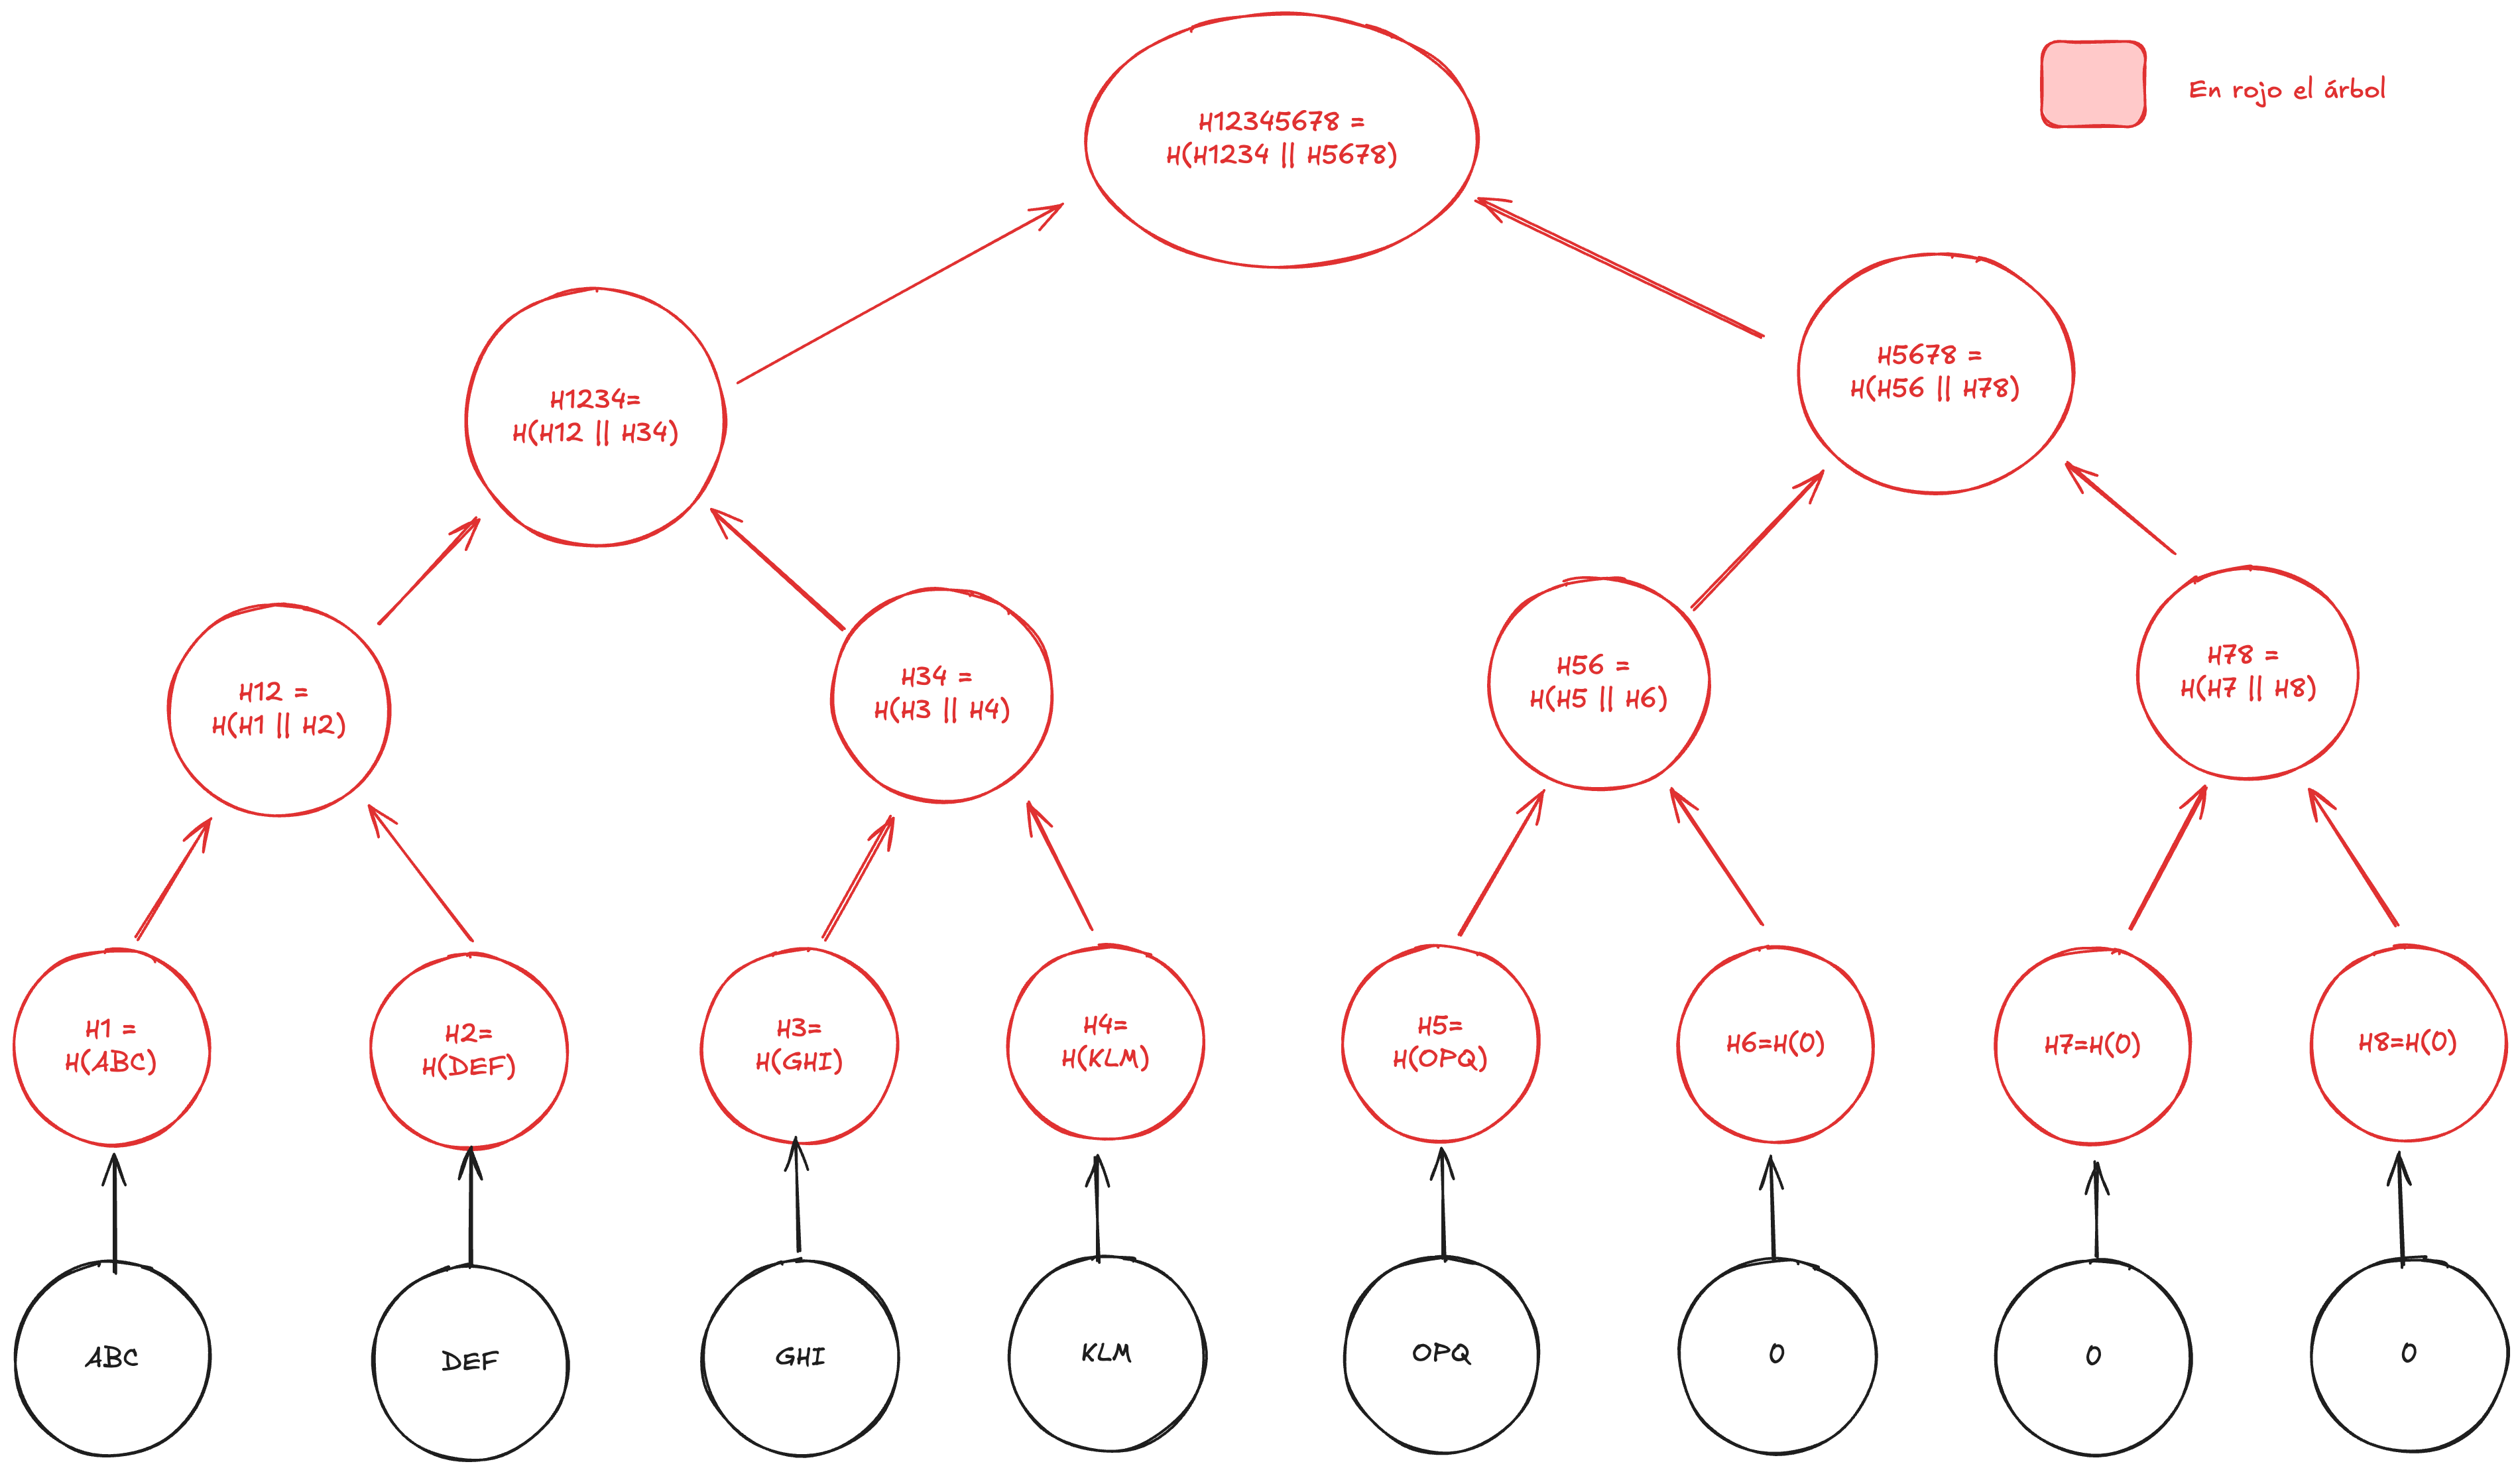
\includegraphics [width=0.8 \textwidth]{mt.png}
        \caption{MT ejercicio 1.b}
    \end{figure}    

    \begin{figure}[h]
        \centering
        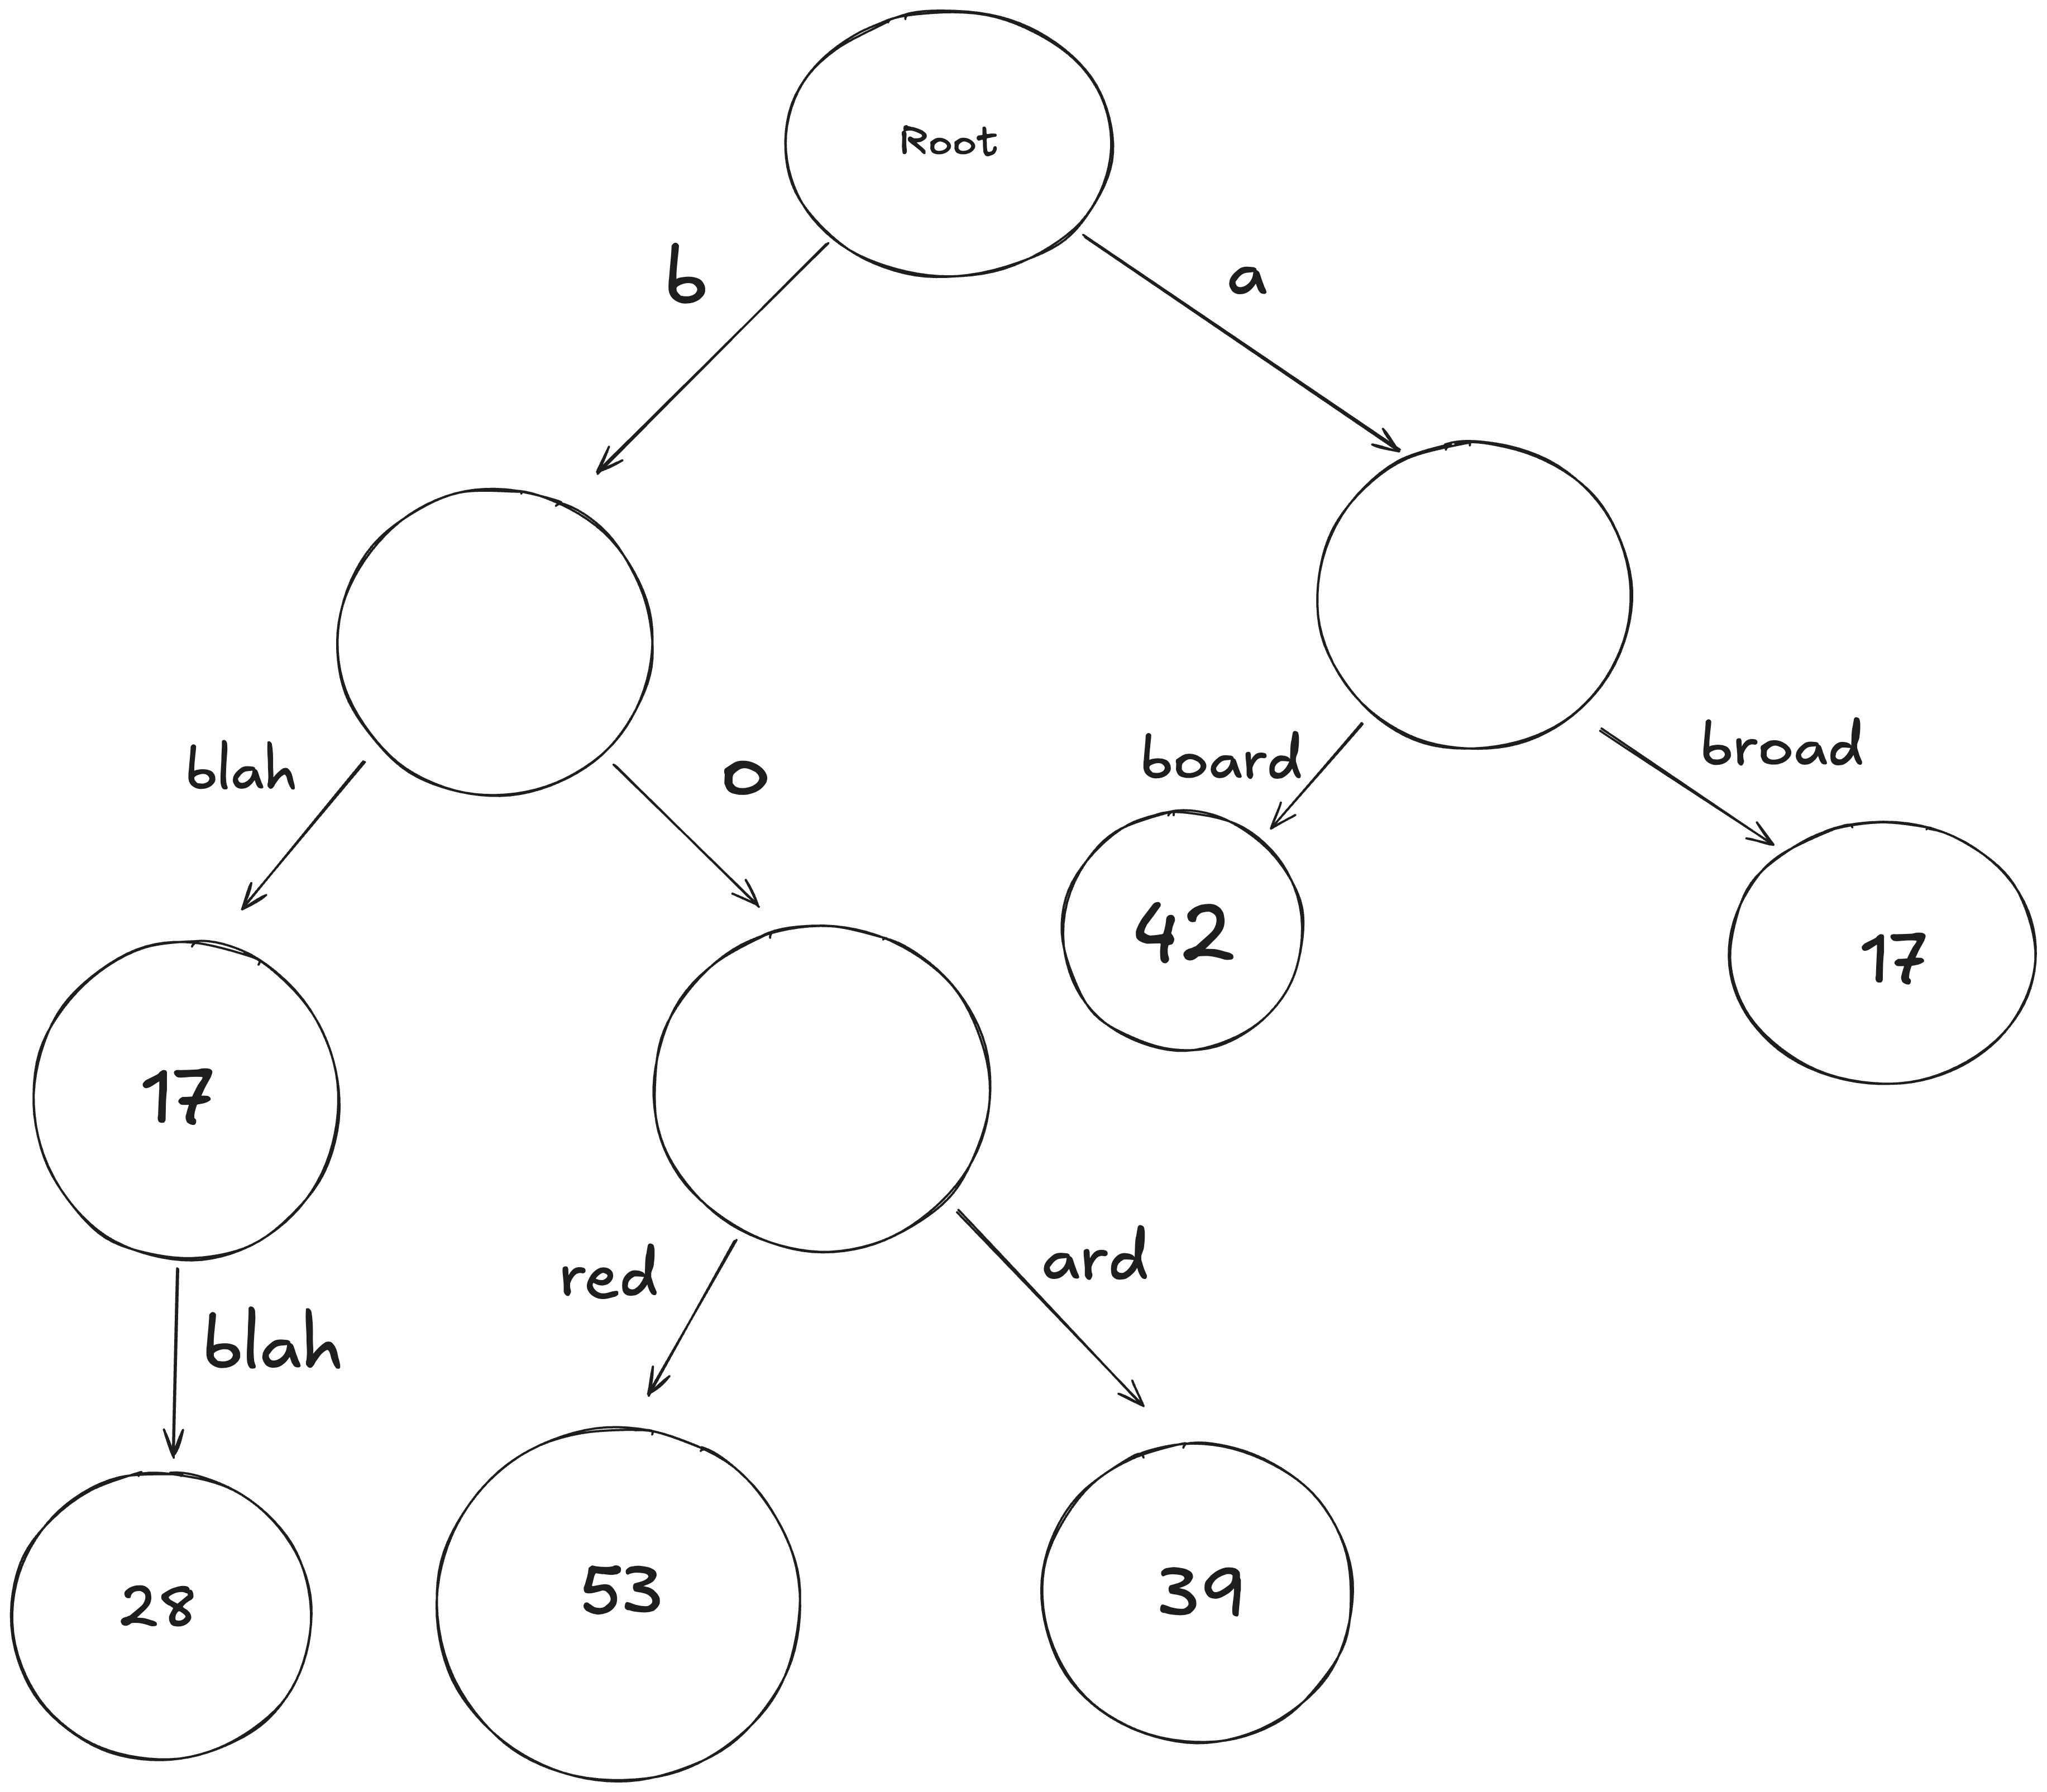
\includegraphics [width=0.8 \textwidth]{pt.png}
        \caption{PT ejercicio 1.c}
    \end{figure} 
\newpage




\question Cryptographic hash functions:

\begin{parts}

\part[5] Derive the formula for the {\em birthday paradox} we saw in class (show your work, explaining every step) and
calculate the number of elements needed to find a collision with at least 50\%. 

\begin{solution} 

    Para este ejercicio me guié usando las diapositivas de la clase dos donde vimos la paradoja del cumpleaños.

    La idea es encontrar cuántas personas son necesarias para que haya al menos 50 porciento de probabilidad de 
    que 2 personas (distintas) cumplan el mismo dia. 
    
    Llamemos A al evento en que dos personas cumplen el mismo dia. 
    Como es mas sencillo calcular la probabilidad de que no haya dos personas que cumplan el mismo dia, 
    notemos $P(B) = P(\lnot A)$, calculemos P(B). Luego, por complemento,  P(A) = 1 - P(B).

    Sea n la cantidad de todas las posibles fechas y k la cantidad de personas:


    La probabilidad de B es casos favorables sobre casos posibles:

    $\textbf{Analizando casos posibles}$:

    Si hay n dias, cada persona tiene para n opciones para cumplir años. Como hay k personas y 
    cada opcion es independiente entonces hay $n^k$ posibilidades.

    $\textbf{Analizando casos favorables}$:
    
    Aca hay que tomar las todas las posibilidades donde no se repiten dias. La primer pesrsona tiene n dias posibles, 
    para que no se repitan la segunda tiene n-1 dias posibles,..., la k-esima tiene n-k+1 dias posibles. Es decir:

    $n \times (n-1) \times ... \times (n-k+1)$
    

    $\textbf{Probabilidad de B}$:


    $P(B) = \frac{n \times (n-1) \times ... \times (n-k+1)}{n^k}$


    $= \prod^{k-1}_{l=1}(\frac{n-l}{n}) = \prod^{k-1}_{l=1}(1 - \frac{l}{n})$ ordeno como productoria


    $\leq exp(-\frac{1}{n} \sum^{k-1}_{l=1} l)$ 

    $= exp(\frac{-k(k-1)}{2n})$

    Para que haya al menos 50\% de probabilidad de que haya una colision necesito $P(B) \leq 0.5$:

    $P(B) \leq \frac{1}{2}$

    $\frac{-k(k-1)}{2n} \leq ln(\frac{1}{2})$ (tomando logaritmo natural de ambos lados)
    
    $k^2 - k \geq 2n ln(2)$

    Usando la resolvente (es una cuadratica) hallamos k:

    $k \geq \frac{1 + \sqrt{1 + 8n ln2}}{2}$
    
\end{solution}  

\part[5] Apply the above result to find out how many Bitcoin users are needed to initialize their wallet’s seed, which is based on a random selection of 12 random words from the list in \url{https://github.com/bitcoin/bips/blob/master/bip-0039/english.txt}, to have the event that, with probability at least 50\%, at least two users end up with exactly the same seed.

\begin{solution} 

    En este caso n va a ser la cantidad de seeds que se pueden formar. Hay 2048 palabras en la lista y cada seed 
    se conforma de 12 palabras, es decir que hay $2048^{12}$ seeds distintas (entendiendo que importa el orden de las palabras
    y pueden repetirse en una misma seed).

    Dicho esto se necesitarian k usuarios con $k = \frac{1+\sqrt{1+8 \times 2048^{12} ln 2}}{2}$
    
    (un numero ridiculamente grande)    
\end{solution}

\end{parts}

\newpage

\question[10] Prof. Gray has designed a cryptographic hash function $H_G : \{0, 1\}^\ast \rightarrow \{0, 1\}^n$. One of his brilliant ideas is to make $H_G(x) = x$ if $x$ is an $n$-bit string (assume the behavior of $H_G$ is much more complicated on inputs of other lengths). That way, we know with certainty that there are no collisions among $n$-bit strings. Has Prof. Gray made a good design decision? Justify your answer, in particular listing the properties that may or may not be satisfied by the design.

\begin{solution} 

    No es una buena idea, desarrollo respecto a las propiedades que debe cumplir una funcion de hash para ser segura:

    \begin{enumerate}
        \item \textbf{Resistencia a colisiones:} 
        Tenemos que garantizar que sea dificil hallar x,x' tal que: H(x) = H(x').
        Con este esta implementacion sea x cualquier string de longitud mayor a n y H(x) = h (h tiene longitud n). Obtener
        x' con el mismo hash es tan sencillo como elegir el string h, pues H(h) = h. Entonces esta funcion de hash no cumple
        con la propiedad de ser resistente a colisiones.

        \item \textbf{Resistencia a la Pre-Imagen}:
        La funcion deberia garantizar que dado y = H(x), para un x cualquiera sea dificil encontrar x' tal que H(x') = y.
        En este caso tambien tenemos problemas si y es un hash cualquiera, hallar x' tal que H(x') = y
        es tan sencillo como elegir el string y (como es el resultado de una funcion de hash su longitud es n). 
        Por como esta definida la funcion va a valer que
        H(y) = y

        \item \textbf{Resistencia a la segunda pre-imagen:} 

        Por lo mismo que explique en el primer punto tampoco es resistente a la segunda pre-imagen, dado un cualquier x 
        de longitud mayor a n, H(x) = h y $|h|$ =  n. Podemos hallar x' que compla H(x) = H(x') tomando simplemente  x' = h.
        

        Se pierden caracteristicas escenciales como que la funcion sea one way, "random" y que cuando cambiamos muy poco
        el contenido a hashear este cambie de manera impredecible.
    \end{enumerate}
\end{solution}

\newpage

\question[10] As we saw in class, the main security notion for digital signatures is called {\em existential unforgeability}, which prevents an attacker from producing a signature on a message that has not been produced by the legitimate signer. I.e., the attacker should not be able to produce the pair $(m, \sigma)$, where $\sigma$ was not produced by the legitimate signer. 

Show an attack on the plain RSA signature scheme we saw in class in which an attacker forges a signature on an arbitrary message $m$ by asking the signer to sign two other different messages (not necessarily unrelated to $m$).

\begin{solution} %Uncomment and type your solution here

    Leí el siguiente artículo para este punto: 
    
    https://www.geeksforgeeks.org/computer-networks/rsa-and-digital-signatures/

    Si un atacante obtiene dos firmas de dos mensajes, es capaz de firmar un m arbitrario.

    Sean los mensajes $m_1, m_2$ sus firmas son:
    
    $s_1= m_1^d$ mod N  y  
    
    $s_2 = m_2^d$ mod N

    respectivamente.

    Para verificar una firma hay que chequear si $s^e$ mod N $= m$

    (Ya que $(m^d)^e$ mod N = m)

    El atacante puede firmar $m = m_1 m_2$ ya que su firma es directamente $s = s_1 s_2$ mod N.


    Veamos que se verifica la firma:

    $s^e \text{ mod N } = 
    (s_1 s_2)^e \text{ mod N } = 
    (m_1^d m_2^d)^e \text{ mod N } = 
    (m_1 m_2)^{d e} \text{ mod N } = \\
    m^{de} \text{ mod N }
    = (m^d)^e \text{ mod N } = 
    m$
\end{solution}

\newpage

\question[10] A Bitcoin miner creates a block $B$ which contains address $\alpha$, on which it wants to receive its rewards. An attacker changes the contents of $B$, such that instead of $\alpha$ it defines a new address $\alpha'$, which is controlled by the attacker. Will the attacker receive the rewards that the miner tries to claim? Why or why not? Give a detailed explanation of your answer.

\begin{solution} %Uncomment and type your solution here

    No, el atacante no va a recibir las recompensas. Si el atacante cambia el contenido del bloque, este va a dejar
    de ser congruente con la cadena ya que el hash depende de su contenido por lo que no va a haber consenso. 
    Para eso esta proof of work, si el atacante quiere cambiar un bloque necesita consenso y para eso tendria que hacer
    la proof of work.

\end{solution}

\newpage

\question[10] Using the course’s Sepolia  Testnet chain, send 0.05 ETH to the address of a fellow student. Describe how you conducted the payment, including the transaction’s id and addresses which you used. (Refer to the Solidity tutorial material “How to Connect
to a Public Testnet” document shared on Campus, as well as the Solidity
tutorial material and pointers.) 

\begin{solution} %Uncomment and type your solution here

    Para este ejercicio escribi un smart contract en solidity con dos funciones. La idea es cargar fondos
    en el contrato y luego poder usar esos fondos para transferir a quien indiquemos.

    \begin{itemize}
        \item fondear contrato: 
        
        Como lo dice su nombre sirve para que fondeemos el contrato.
        Es importante que sea payable para poder enviar eth en la transacción.
        \item transferir: 
        
        Esta función envía a 
        destinatario el monto indicado, usando los fondos del contrato. (la direccion debe ser payable porque le
        vamos a enviar eth)


        Primero llamé a la función fondear para enviarle 0.05 eth (expresado en wei) al contrato y luego use
        la funcion transferir para enviar esos eth a mi compañero

        direccion del contrato: 0xf4d279F94919d3389ff3ba09f73c370cf37D7F55

        mi direccion: 0x65De8AcFCC18B4D182857Cf19c687AF735Ffc9CD
        
        direccion de mi compañero: 0xC57f1Cb50Ec19B8735ea28a6d84AEe85f0d88c07
        
        transaccion fondeo del contrato: 
        
        0x9e7bddbea7c49ec041893743b812023f3875ec7755a28eedbd66f85e6e3154b7
        
        transaccion envío: 

        0xe631331b42a31b1de9fa4f2d1dec4fed969fc6e9d343f3a6c89636a6d096d0cc 

    \end{itemize}
    
\end{solution}
\begin{verbatim}

    // SPDX-License-Identifier: GPL-3.0

    pragma solidity >=0.7.0 <0.9.0;

    contract Transfer{
        
        function fondear_contrato() public payable {} 

        function transferir(address payable destinatario, uint monto) public{
            require(address(this).balance >= monto, "Fondos insuficientes");
            destinatario.transfer(monto);
        }
    }

\end{verbatim}

\newpage
  
\question The following smart contract has been deployed on the Sepolia Testnet chain:

{\footnotesize

\begin{verbatim}
// SPDX-License-Identifier: GPL-3.0

pragma solidity >=0.7.0 <0.9.0;

contract Bank {
    mapping(address => uint256) balance;
    address[] public customers;

    event Deposit(address customer, string message);
    event Withdrawal(address customer);

    function deposit(string memory message) public payable {
        require(msg.value > 10);
        balance[msg.sender] += msg.value - 10;

        customers.push(msg.sender);

        emit Deposit(msg.sender, message);
    }

    function withdraw() public {
        uint256 b = balance[msg.sender];
        balance[msg.sender] = 0;
        payable(msg.sender).transfer(b);

        emit Withdrawal(msg.sender);
    }

    function getBalance() public view returns (uint256) {
        return balance[msg.sender];
    }
    
    function empty() public {
        require(msg.sender == customers[0]);
        
        payable(msg.sender).transfer(address(this).balance);
    }
}
\end{verbatim}

} %FOOTNOTESIZE

 Its deployed address is: 0x4310a5f4Bb3b4Ff09f0694218fA50D2767a00b86. You can compile it and interact with it using Remix. You should successfully create a transaction that interacts with the contract, either depositing or withdrawing from it some coins. 
 
 \begin{parts} 
 
 \part[5] Describe the contract’s functionality (that is, the purpose of each variable, function, and event).
 
\begin{solution} 

    El contrato modela el comportamiento de un banco.

    La primera variable balance es un mapping (se puede pansar como un diccionario key/value) que mapea direcciones (address) a 
    numeros positivos (su balance). Basicamente guarda el balance de cada cliente.

    Customers es un arreglo de addresses, contiene a los clientes del banco.

    Luego define dos eventos, Deposit y Withdrawal. Estos los podemos emitir, avisando que un cliente deposito o retiro balance
    del banco. Los event no modifican el estado del contrato pero si quedan registrados en la blockchain.

    La funcion deposit requiere que la cantidad de eth de quien la llama sea mayor a 10. 
    Luego le suma a su balance ese valor restandole 10 (imagino que es una especie de comision). 
    Despues agrega al cliente a la lista de clientes y por ultimo emite el evento
    deposit, indicandoque ese cliente envio ese mensaje. Notar que la funcion es payable por eso quien la llama puede gastar eth.
    
    La funcion withdraw se guarda en una variable local el balance de quien la llamo. Setea su balance en el map del 
    contrato como cero y luego le transfiere los eth correspondientes.
    Por ultimo emite el evento Withdrawal indicando que es cliente realizo un retiro.

    La funcion getBalance simplemente devuelve el balance que esta guardado en el map de quien llamo a la funcion. Es view
    porque no modifica el estado del contrato simplemente lee variables.

    La funcion empty requiere que quien la llama sea el customer que esta en la possicion inicial del array de customers.
    Le transfiere todo el balance del contrato (el balance de la address no del map) a quien llamo a la funcion.


\end{solution}


\part[15]
 
 Provide the id of the transaction you performed and the address you used.
 
    \begin{solution} 

        Mi address es: 0x65De8AcFCC18B4D182857Cf19c687AF735Ffc9CD
        
        id de transaccion:
        
        0x306edc7f4205d6a3d470b8ae5931ee31ebd48ada820509360dea5fa234829f65
    \end{solution}

\end{parts}

\newpage

~\\

\end{questions}

\end{document}
